\section{Formalização e o Modelo de Mendel}

\begin{frame}{Definindo as Hipóteses}
    \begin{block}{Hipótese Nula ($H_0$)}
        Afirma que a variação observada nos dados é apenas fruto do acaso e não de uma causa sistemática. Sob essa hipótese, conseguimos simular computacionalmente a geração dos dados.
    \end{block}
    \begin{block}{Hipótese Alternativa ($H_1$)}
        Afirma que há um fator sistemático que gerou o desvio dos dados. A variação não pode ser explicada apenas pelo acaso.
    \end{block}
    \begin{alertblock}{Estatística de Teste}
        É a métrica quantitativa usada para avaliar quão longe os dados observados estão daquilo que é previsto pela hipótese nula $H_0$.
    \end{alertblock}
\end{frame}

\begin{frame}{Entendendo o P-Valor (Valor de Probabilidade)}
    \begin{block}{Definição Oficial}
        P-valor é a probabilidade de observar um valor de estatística de teste tão extremo ou mais extremo do que o observado, sob a premissa de que a Hipótese Nula $H_0$ é verdadeira.
    \end{block}
    \begin{alertblock}{Erros Comuns de Interpretação}
        \begin{itemize}
            \item \textbf{NÃO É} a probabilidade de a hipótese nula ser verdadeira.
            \item \textbf{NÃO É} a probabilidade de a hipótese alternativa ser falsa.
            \item É apenas um medidor de surpresa sob a hipótese nula.
        \end{itemize}
    \end{alertblock}
\end{frame}

\begin{frame}{Estudo de Caso: O Modelo de Genética de Mendel}
    \begin{block}{Mendel e a Hereditariedade das Plantas}
        Gregor Mendel propôs que em cruzamentos híbridos, a planta tinha $75\%$ de chance de ter flores roxas e $25\%$ de ter flores brancas.
    \end{block}
    \begin{columns}
        \begin{column}{0.5\textwidth}
            \textbf{Os Dados Observados:}
            \begin{itemize}
                \item Tamanho da amostra ($N$): $929$ plantas.
                \item Plantas de flor roxa: $705$ ($\approx 75.89\%$).
                \item Desvio observado: $0.89\%$.
            \end{itemize}
        \end{column}
        \begin{column}{0.5\textwidth}
            \centering
            \textit{Será que o desvio de $0.89\%$ da previsão de $75\%$ é sinal de falha do modelo de Mendel ou apenas ruído amostral?}
        \end{column}
    \end{columns}
\end{frame}

\begin{frame}{Matemática do Exemplo de Mendel}
    \begin{block}{Estatística de Teste: Distância Absoluta}
        Como há apenas duas categorias, a estatística de teste ideal é a diferença absoluta entre o percentual observado e $75\%$:
        $$\text{Estatística} = \left| \text{Percentual de Flores Roxas} - 75 \right|$$
    \end{block}
    \begin{block}{Cálculo do Valor Observado}
        $$\text{Percentual Observado} = \frac{705}{929} \times 100 \approx 75.888\%$$
        $$\text{Estatística Observada} = \left| 75.888 - 75 \right| = 0.888\%$$
    \end{block}
\end{frame}

\begin{frame}[fragile]{Abordagem Computacional: Mendel}
\begin{lstlisting}[language=Python]
import numpy as np

tamanho_amostra = 929
prob_roxa = 0.75
repeticoes = 10000

# Simula 10000 experimentos sob a hipotese nula
np.random.seed(42)
simulados = np.random.binomial(n=tamanho_amostra, p=prob_roxa, size=repeticoes)
percents_simulados = (simulados / tamanho_amostra) * 100
estatisticas_sim = np.abs(percents_simulados - 75.0)

# Calcula o P-valor
obs_dist = np.abs((705 / tamanho_amostra) * 100 - 75.0)
p_valor = np.count_nonzero(estatisticas_sim >= obs_dist) / repeticoes
print(f"P-valor: {p_valor:.4f}")
# Saida aproximada: 0.5418
\end{lstlisting}
\end{frame}

\begin{frame}{Mendel: Decisão Visual}
    \begin{columns}
        \begin{column}{0.5\textwidth}
            \textbf{Análise do Resultado:}
            \begin{itemize}
                \item O desvio de $0.888\%$ ou maior ocorre em mais de $54\%$ das simulações aleatórias.
                \item O desvio observado é comum no mundo nulo.
                \item \textbf{Decisão:} Não rejeitamos a hipótese nula $H_0$. O modelo de Mendel é consistente com os dados.
            \end{itemize}
        \end{column}
        \begin{column}{0.5\textwidth}
            \centering
            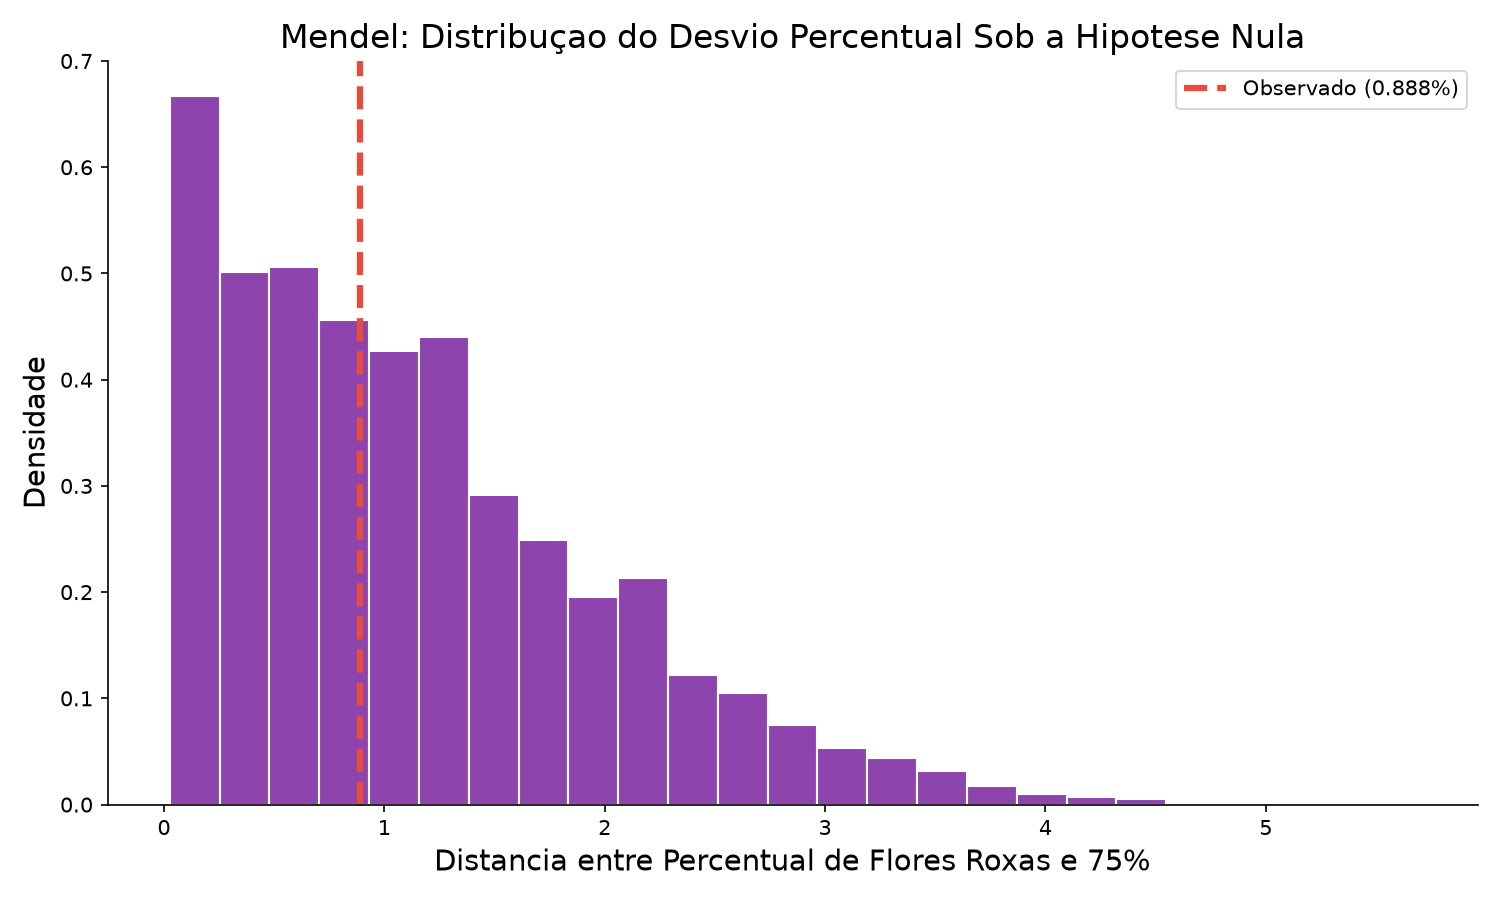
\includegraphics[width=\textwidth]{03_mendel_histograma.png}
        \end{column}
    \end{columns}
\end{frame}
